\section{Confidence Sets}
\frame{
\frametitle{}
\begin{block}{}
\centering
Confidence Sets for Persistence Diagrams:\\
Analyzing Descriptors
\end{block}
}



\frame{
\frametitle{Objective}
\framesubtitle{~}

\begin{block}{To Find a Threshold}
 Given $\alpha \in (0,1)$, we will find $q^{\alpha}$ such that
  $$\mathbb{P}(
  W_{\infty}(D,\widehat{D}_n) \leq q^{\alpha}
) \geq 1-\alpha.$$
\end{block}
\pause
\begin{block}{References}
    \begin{itemize}
        \item BTF, Lecci, Rinaldo, Wasserman, Balakrishnan, and Singh.
            Confidence sets for persistence diagrams. Annals of Stat., 2014.
        \item Chazal, Lecci, BTF, Rinaldo, Singh, and Wasserman.
            On the Bootstrap for Persistence
            Diagrams and Landscapes.
            Modeling and Analysis of Information Systems, 2013.
        \item Chazal, BTF, Lecci, Michel, Rinaldo, and Wasserman.
            Robust Topological Inference: Distance To a Measure and Kernel
            Distance, JMLR, to appear.
    \end{itemize}
\end{block}
}

\frame{
    \todo{add a few slides on the Bootstrap technique in general}
}

\begin{frame}
    \frametitle{Bottleneck Bootstrap}

    \begin{columns}
        \column{.45\textwidth}

        \begin{block}{}
            We have one sample: $\mathcal{S}_n = \{ X_1, \ldots, X_n\}$; $X_i \sim P$.
        \end{block}

        \pause

        \begin{block}{}
            Subsample (with replacement), obtaining:
            $X = \{ X_1^*, \ldots, X_b^*\}$
        \end{block}

        \pause

        \begin{block}{}
            Compute
            $\hat{\Theta}_b^*(X^*) =
            W_{\infty}(X^*,\mathcal{S}_n)$ using KDE or DTM.
        \end{block}

        \column{.45\textwidth}
        \centering
        \only<4-5>{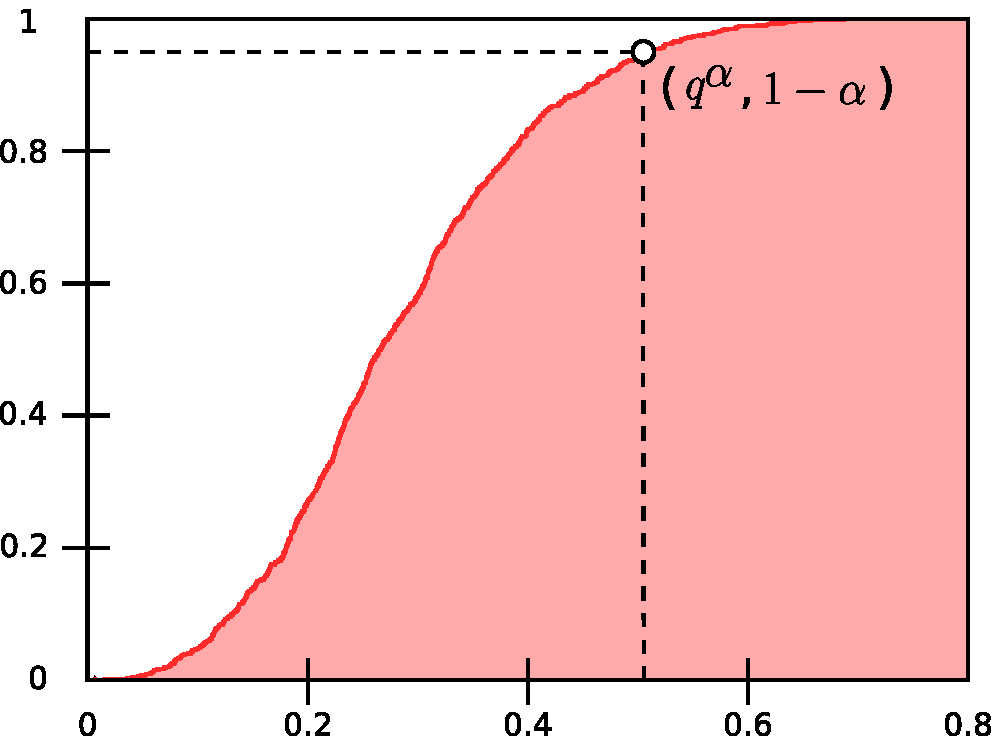
\includegraphics[height=1.6in]{stat/cdf-full}}
        \only<6->{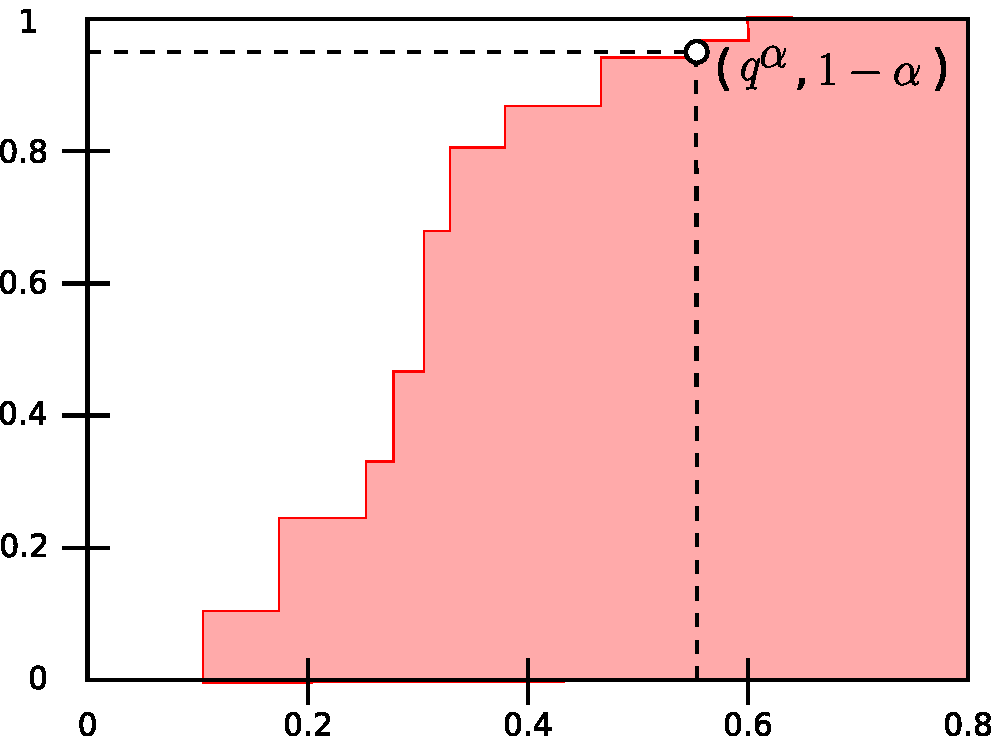
\includegraphics[height=1.6in]{stat/cdf-estimate}}

    \end{columns}

    \pause
    \begin{columns}
        \column{.45\textwidth}
        \begin{block}{}
            Consider all possible outcomes:
            $$ \{ \hat{\Theta}_{b}^*(X^*) \}_{X^* \subset \mathcal{S}_n}$$
        \end{block}

        \column{.45\textwidth}
        \pause
        \begin{block}{}
            Mimics:
            $$ \{ {\Theta}(X) = W_{\infty}(\mathcal{S}_n,\mathbb{M}) \}_{\mathcal{S}_n
            \subset \mathbb{M}}$$
        \end{block}
    \end{columns}
\end{frame}



\begin{frame}
 \frametitle{Confidence Sets for Persistent Diagrams}
 \framesubtitle{~}
 % side by side figures
 \begin{block}{}
  $$C_{\alpha}
  = \{ D \in \mathcal{D}_T ~:~ W_{\infty}(D,\widehat{D}_n) \leq q^{\alpha} \}$$
 \end{block}

 \begin{columns}
  \column{.45\textwidth}
     \begin{figure}
     \centering

 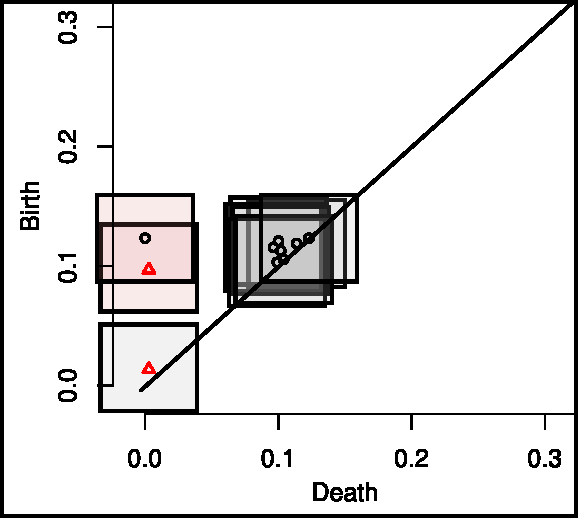
\includegraphics[height=1.6in]{stat/eyeglasses-density-pers-Point-ci.pdf}
     \end{figure}
  \column{.45\textwidth} \pause
     \begin{figure}
     \centering

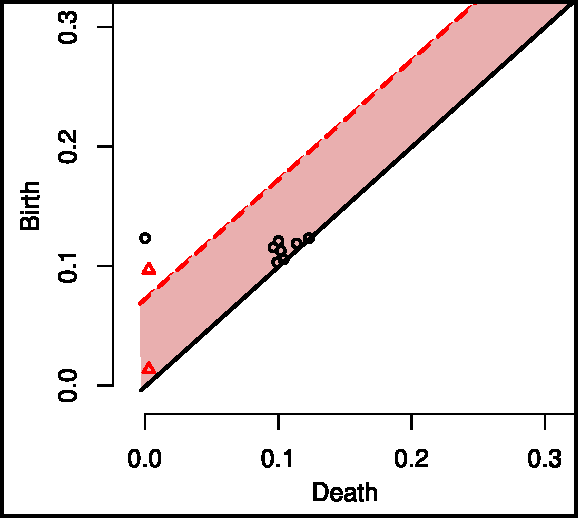
\includegraphics[height=1.6in]{stat/eyeglasses-density-pers-CI.pdf}
     \end{figure}
\end{columns}
\end{frame}

\frame{
    \frametitle{Example}

    \begin{block}{}
        \centering
        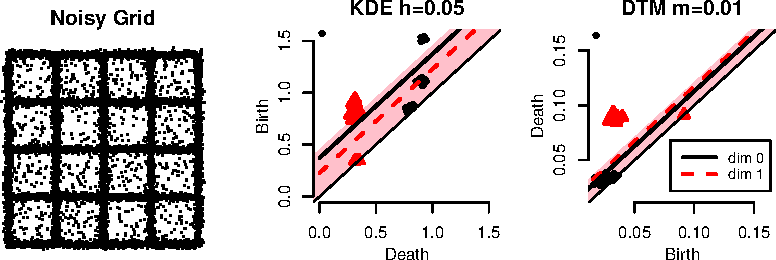
\includegraphics[width=\textwidth]{stat/noisy-grid2}
    \end{block}
}


\frame{
\todo{add a slide about Bootstraps + technical challenge}
}
